\documentclass[english]{oegatb}
\usepackage[utf8]{inputenc}
\usepackage[T1]{fontenc}
\usepackage{eurosym}
\usepackage{tabularx}
\usepackage{graphicx}
\usepackage{float}

\title{Titel}

\author{Erste Autorin, Zweiter B. Autor, und Dritte C. Autorin}

\affiliation{%
Erste A. Autorin ist am Institut für Agrar- und Forstökonomie
der Universität für Bodenkultur tätig (erste.autorin@boku.ac.at).

Zweiter B. Autor arbeitet bei der Aarhus University,
Department of Biology, DK-8000, Aarhus, Dänemark.
Er ist nun bei der Danish Research Centre of Organic Food and Farming,
DK-8830 Tjele, Dänemark tätig (secondb.author@agrsci.dk).

Dritte C. Autorin ist an der University of Copenhagen,
Department of Zoology, Denmark (thirdc.author@agrsci.dk).}


\begin{document}
\maketitle

\begin{abstract}
These instructions give you guidelines for preparing camera-ready short papers
for the ÖGA 2006 conference proceedings.
The short papers can be written in German or in English.
The length of the short paper is maximally two pages.
There will be no key words.
Use this document as a template if you are using Microsoft Word 6.0 or later.
Otherwise, use this document as an instruction set. Define all symbols
used in the paper.
Do not cite references in the abstract.
The abstract should not exceed ca.\ 200 words, which corresponds
to the double length of this example.
The footnote symbol following this abstract should not be deleted.
\end{abstract}


\section{Introduction to using the template}

This document is a template for Microsoft Word versions 6.0 or later.
If you are reading a paper version of this document,
please download the electronic file, template.doc,
from the website \url{http://www.boku.ac.at/oega} so you can use it
to prepare your manuscript.

When you open the template, select ‘Page Layout’ from the ‘View’ menu
in the menu bar (View | Page Layout),
which allows you to see the footnotes.
Then type over the sections or cut and paste from another document
and then use markup styles.
The pull-down style menu is at the left of the Formatting Toolbar
at the top of your Word window.
For example, the style at this point in the document is ‘Normal text’.
Highlight a section that you want to designate with a certain style,
and then select the appropriate name on the style menu.
The style will adjust your fonts and line spacing.
Styles used are: title, author, abstract, normal text, heading 1
(as in ‘introduction above) and footnote.
Subheadings (as ‘Figures and tables’ in next column are italicized normal text.
Do not change the font sizes or line spacing to squeeze more text
into a limited number of pages.
Use italics for emphasis; do not underline.
Please note that there is a tab at the beginning of each paragraph,
except for the first paragraph in a section.


\section{Procedure for paper submission}

Papers must be submitted by 31st August 2006 per email to
\url{michaela.groetzer@boku.ac.at}.
Papers received after this deadline cannot be included in the proceedings.
Paper exceeding 2 pages can also not be included in the proceedings.
The submitted paper must be in camera-ready format and in a word file.
It will be placed into the conference proceedings as received
and without substantial editing or reviewing.
Therefore, we recommend that you get one or two colleagues
to proofread the paper.


\section{Structure of the short paper}

The short paper should be structured as any other scientific publication.
You should start with an introduction which includes background information
(why is the topic of your research relevant?
What have other authors found out about the topic?)
and the specific question you tried to answer in your study
(what is your aim and/or hypothesis?).

The second section should explain the methods you used,
so that the readers have clear information on how (and where)
the data was collected and what methods were used to analyse the data.

The third section should present the results of your research,
i.e.\ describe your major findings.
Please try to be as succinct as possible,
presenting only the most relevant data in condensed form.

In the fourth section you should explain how you interpret your results
(do not leave the reader thinking "So what?").
Continually refer to your results (but do not repeat them).
Do not extend your conclusions beyond those
which are directly supported by your results.
Speculation has its place, but should not form the bulk of the discussion.
Be sure to address the objectives of the study
(which you stated in the introduction).
Discuss the significance of your results in light of other published work.
End the discussion with a short summary or conclusion
regarding the significance of the work.


\section{Helpful hints on formatting}

\subsection{Figures and tables}
As there will be no final formatting of your paper,
you need to place figures and tables in the paper accordingly,
usually at the top or bottom of column.
Large figures and tables may span both columns,
but it is easier to include a one-column figure or table.
Place figure captions below the figures; place table titles above the tables.

\begin{table}[H]
\caption{Soil properties for the two studied soils
(Style used is Normal text, but font size 7).}
\scriptsize
\renewcommand{\arraystretch}{1.1}
\begin{tabularx}{\columnwidth}{Xcc}
\hline
Soil property     & Soil A & Soil B\\
\hline
Temperature (C)   &     15 &     12\\
pH                &    7.4 &    6.2\\
Organic C (mg/kg) &    1.2 &    2.4\\
\hline
\end{tabularx}\\
\textsuperscript{a} Water content is given on a soil dry weight basis.
\end{table}

Please verify that the figures and tables you mention in the text
actually exist. Please do not include captions as part of the figures.
Do not put captions in text boxes linked to the figures.
Do not put borders around the outside of your figures.
Use the abbreviation ``Fig.'' except at the beginning of a sentence,
where ``Figure'' should be used.
Do not abbreviate ``Table.''
Tables are numbered with Roman numerals.
Insert tables by use of the Table lay-out, not just as tabulated text and data.

Figure axis labels are often a source of confusion.
Use words rather than symbols.
As an example, write the quantity ``Transport cost in \euro'', not just ``\euro''.
Put units in parentheses.
Do not label axes only with units.

Figure labels should be legible, approximately 8 point type.
Color printing of figures is not available.

\subsection{Numbers}
Figures are used for all units and quantities (e.g., 8 mm, 3 years, 6 kg)
with a space between the figure and the measurement description.
In descriptive text, numbers from one to nine are spelled out
and figures are used for 10 and over (e.g., six pigs, 27 sows)
except where the number begins a sentence,
thus: ``Three years ago ....''.
If you use percentages, please do not include a space between the number
and the percentage sign (e.g. 20\% of farmers).

\subsection{Abbreviations and Acronyms}
Define abbreviations and acronyms the first time they are used in the text.
Do not use abbreviations in the title unless they are unavoidable.

\subsection{Data and units}
Indicate which measure is being used when data are presented;
e.g., 53.8 $\pm$ 1.5 g/L (mean $\pm$ SE).
For tests of significance, use the form, e.g., ``P<0.001''.

Use of SI units is strongly encouraged.
Use the center dot to separate compound units (A$\cdot$m2).

\subsection{Tense}
If you wish, you may write in the first person singular
or plural and use the active voice
(``We observed that...'' instead of ``It was observed that ...'' or
``The authors observed that...'').
Remember to check spelling.
If your native language is not English or German
(depending on the language you write in),
please get a native speaker to proofread your paper.


\section{Guidelines for references}

\subsection{In text}

In the body of the text,
references should be cited according to the following rules.\\
- Where a paper is by three or more authors,
  the name of the first author should be followed by et al.\
  [\citet{hansen04} demonstrated\ldots] or
  [as previously demonstrated \citep{hansen04}].\\
- Please place a comma between the author's name and the year
  \citep{schulze94,hansen95}.
  - The earliest work is reported first.\\
- Letters following the year are used to differentiate between
  two or more papers with the same authors and the same year
  (Smith, 1964a, 1964b).\\
- A semi-colon separates reference to different authors
  \citep{schulze94,hansen04}.

\begin{figure}[H]
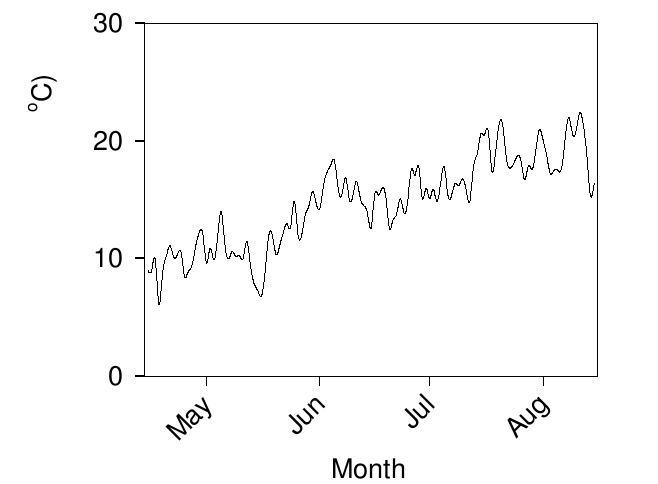
\includegraphics[width=0.9\columnwidth]{oegatb-ex.png}
\caption{Air temperature during the summer in Denmark
(Style as normal text, but in italic and font size 7).}
\end{figure}


\subsection{Reference list}
A complete list of the references cited in the text must be arranged
alphabetically at the end of your paper under the heading References.

For papers published in journals: Authors' names, year of publication,
title of paper, name of journal (in full and italics), volume number (issue),
and the first and last page numbers should be given, in that order.

For books: Authors' names, year of publication, title of book (in italics),
volume or edition number, place of publication and name of publisher
should be given in that order.

For chapters in a book: Authors' names, year of publication, title of chapter.
In: editors. Title of Book (in italics), first and last page,
place of publication and name of publisher.

For a thesis: The author's name, year of publication, title of the thesis,
degree and University should be given, in that order.

There is a 4 pt space between references (4pt before each paragraph).


\section{Acknowledgement}

I would like to thank the Joint Organic Congress for providing
this template and most of the detailed instructions included in it.

\nocite{*}
\bibliography{oegatb-ex}

\end{document}
